%!TEX root = ../../../exa-ma-deliverables.tex
\ApplicationFicheHeading{app-composyx-diffusion}
\label{sec:app:specs:app-composyx-diffusion}
% Generated by scripts/sync_applications.py; edit the CSV snapshot.
\begingroup
\small
\begin{longtable}{@{}>{\raggedright\arraybackslash}p{0.26\textwidth}>{\raggedright\arraybackslash}p{0.69\textwidth}@{}}
\toprule
\textbf{Field} & \textbf{Catalogue value} \\
\midrule
\endhead
id & app-composyx-diffusion \\
name & Diffusion, 3D, weak scaling \\
Partners & Inria BXSO \\
PC & PC1 - ExaMA \\
Responsible (Permanent) & G. Marait \\
WP7 Engineer & \todo[app-composyx-diffusion / WP7 Engineer]{Sheet field missing.} \\
work\_package & WP3 \\
application\_type & demonstrator \\
purpose & Weak scalability of an unstructued FEM heterogeneous diffusion equation in a
3D stratified medium. \\
Method-Algorithm WP1 & finite element \\
Method-Algorithm WP3 & domain decomposition methods \\
inputs & \todo[app-composyx-diffusion / inputs]{Sheet field missing.} \\
outputs & \todo[app-composyx-diffusion / outputs]{Sheet field missing.} \\
metrics & weak-scalability, gpu-acceleration \\
status & benchmark-ready \\
Benchmark scope & solver-scaling, multi-node, multi-gpu \\
Framework & Composyx \\
parallel\_framework & MPI, Multithread, GPU - Cuda, GPU - ROCm \\
repo\_url & \todo[app-composyx-diffusion / repo\_url]{Sheet field missing.} \\
tex\_url & \todo[app-composyx-diffusion / tex\_url]{Sheet field missing.} \\
\bottomrule
\end{longtable}
\endgroup


\subsection{Description of the benchmark}

\label{sec:app:specs:app-composyx-diffusion}

We use the Finite Element Method (FEM) with Q1 elements to solve a
heterogeneous diffusion equation $\nabla \cdot (k \nabla u) = 1$ in a
3D stratified medium. The domain is discretized on a regular mesh, and
then divided into $n_{sd}$ identical subdomains along the first axis.
Along the second axis, it is divided into 10 layers of alternating
conductivity k = 1 and k = 1000. A Dirichlet boundary condition is
applied on the left of the domain (x = 0), a Neumann condition on
every other boundary.

\begin{figure}
  \centering
  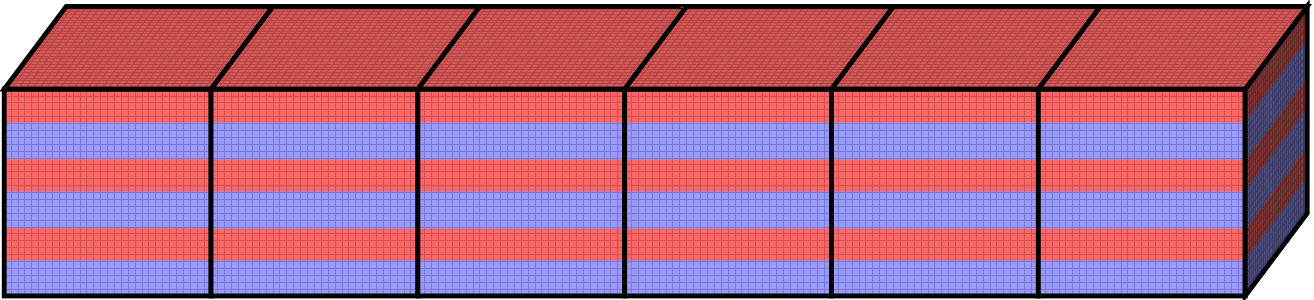
\includegraphics[width=0.8\textwidth]{graphics/composyx/baton.png}
  \caption{Illustration of the composyx-diffusion benchmark test case}
  \label{fig:composyx-baton}
\end{figure}

Each subdomain consists in $60 \times 60 \times 60 = 216 000$
unknowns. Interfaces between two adjacent subdomains have
$60 \times 60 = 3 600$ unknowns. Benchmark in \textbf{weak scaling}
(subdomains are stacked on along an axis). We use one subdomain per
GPU, $n_{sd} = n_{GPU}$. If the GPU has several \textit{Graphics Compute Die} (GCD),
we use one subdomain per GCD.

\begin{table}[ht]
    \centering
    \renewcommand{\arraystretch}{1.1}
    \setlength{\tabcolsep}{4pt}
    \begin{tabular}{|c|c|c|c|c|c|c|c|c|c|}
        \hline
        $n_{\mathrm{sd}}$ & 4 & 8 & 16 & 32 & 64 & 128 & 256 & 512 & 1024 \\
        \hline
        Nb. dofs & 853 200 & 1.7M & 3.4M & 6.8M & 13.6M & 27.2M & 54.4M & 108.8M & 217.5M \\
        \hline
        Schur & 10 800 & 25 200 & 54 000 & 111 600 & 226 800 & 457 200 & 918 000 & 1.8M & 3.7M \\
        \hline
    \end{tabular}
    \caption{Number of total degrees of freedom and size of the Schur
      complement depending of the number of subdomains}
\end{table}

\subsection{Benchmarking methodology}

\paragraph{}
We measure the time spent in each part of Composyx to solve the sparse
linear system using domain decomposition methods on the Schur
complement. We test several preconditioners:

\begin{itemize}
\item \textit{0} for no preconditioner
\item \textit{AS} for Additive Schwarz
\item \textit{NN} for Neumann-Neumann
\item \textit{RR} for Robin-Robin
\item \textit{ASG+} for Additive Schwarz with additive Geneo
\item \textit{ASGd} for Additive Schwarz with deflated Geneo
\item \textit{NNGd} for Neumann-Neumann with deflated Geneo
\end{itemize}

\subsection{Input/Output Dataset Description}
\todo[app-composyx-diffusion / input-output datasets]{Document the benchmark
configuration files, matrix-generator invocation and output data formats.}

\subsection{Results summary}

\subsubsection{Scalability results with HIP}

Composyx was benchmarked on CINES's Adastra supercomputer. Notice that
\textbf{guix} is available of Adastra and HIP software stack, based on
open-source code from AMD was therefore quite easy to deploy.

\begin{figure}
  \centering
  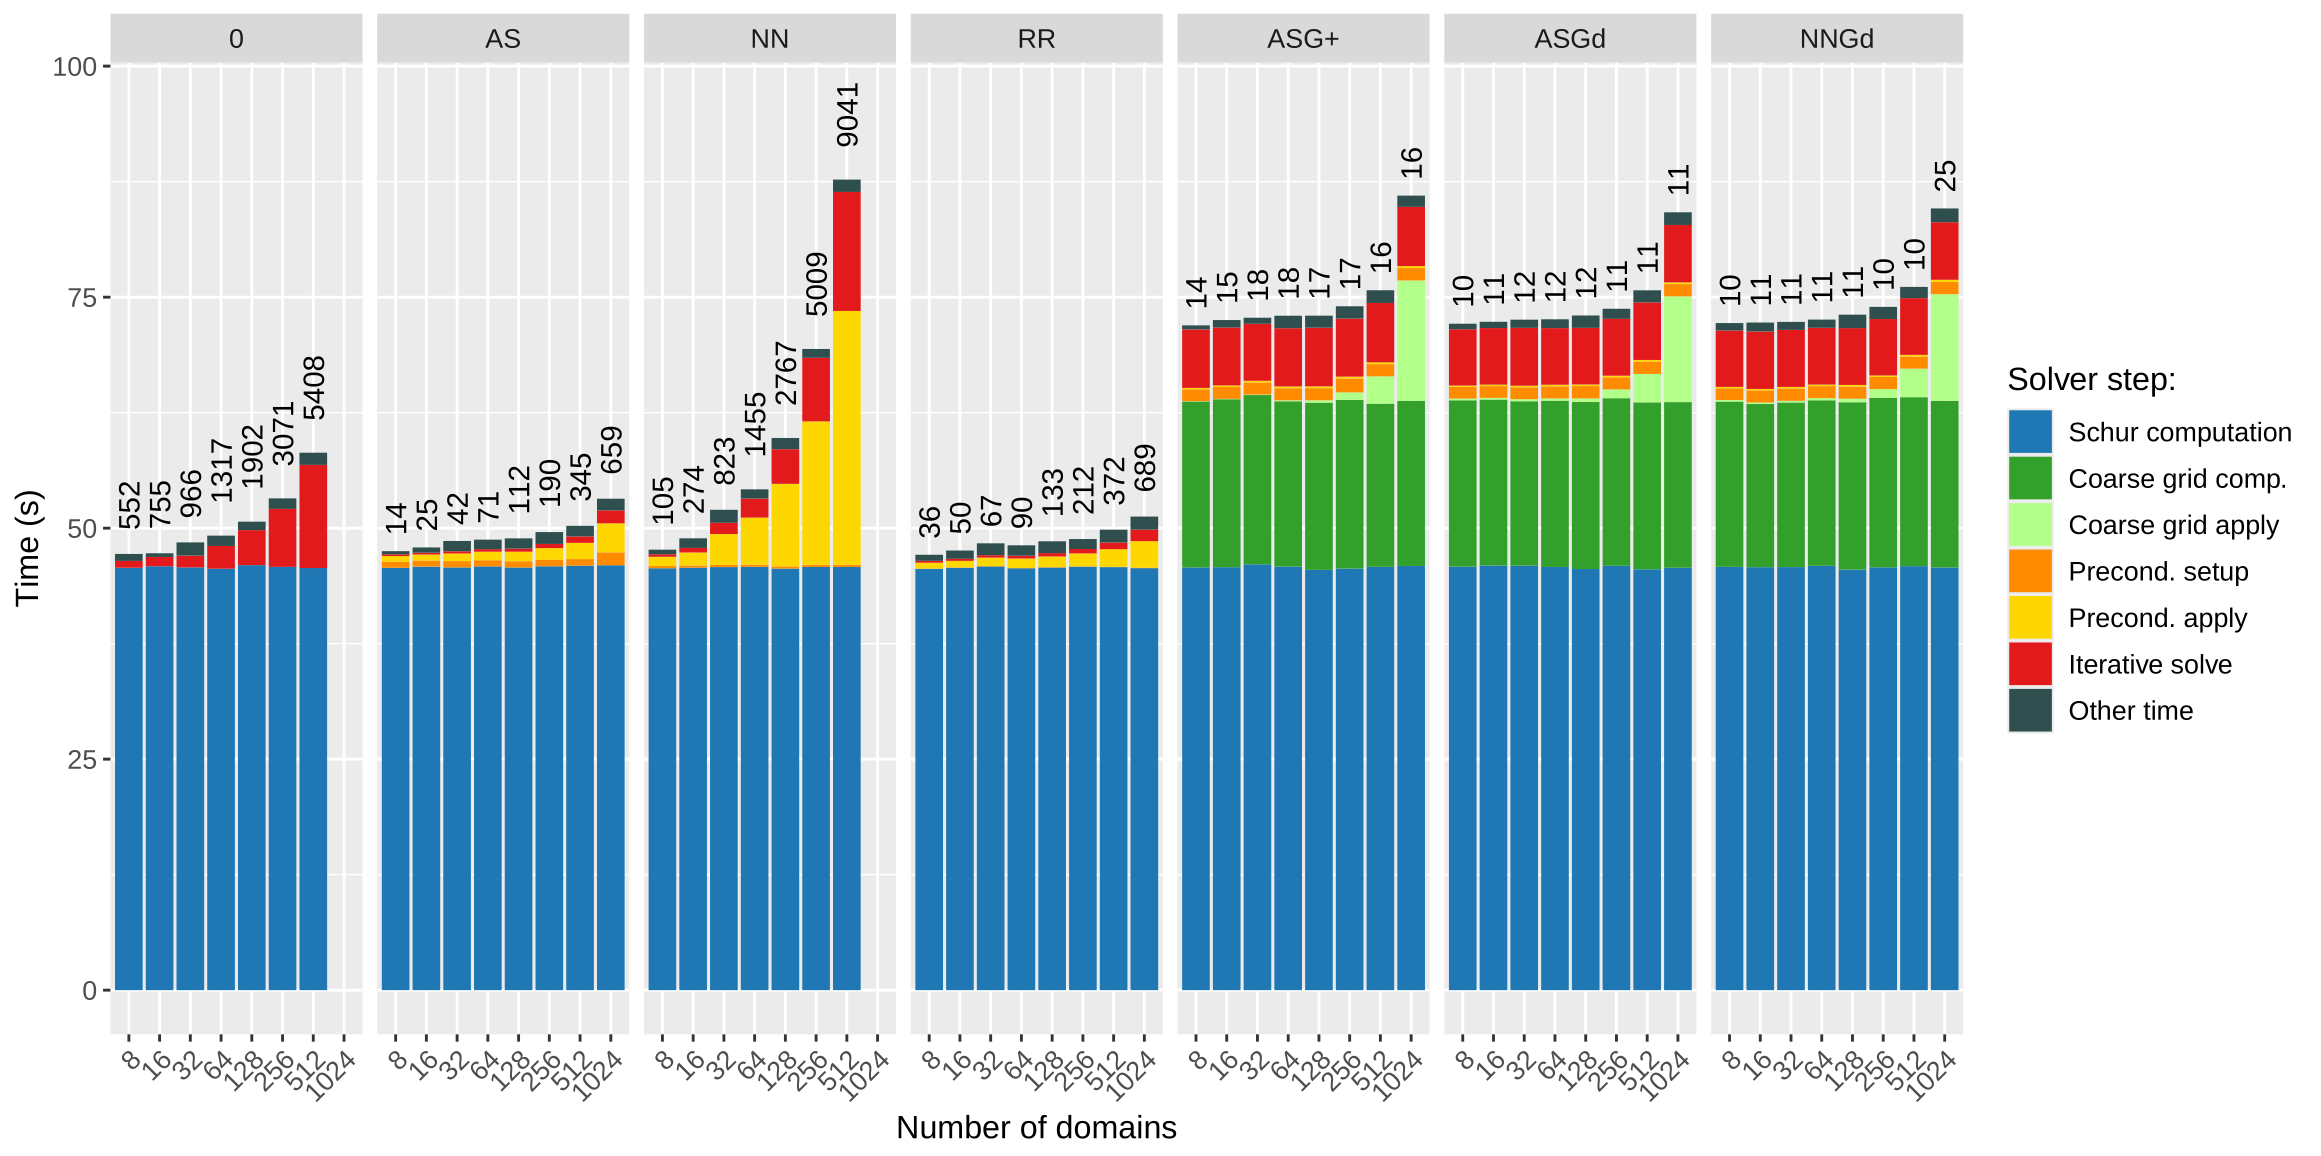
\includegraphics[width=0.8\textwidth]{graphics/composyx/results_adastra_S.png}
  \caption{Composyx weak scaling on Adastra}
  \label{fig:composyx-adastra}
\end{figure}

On Figure \ref{fig:composyx-adastra} are the scaling results from 1 to
128 nodes. The stopping criterion for this experiment is
$\frac{||b - A x ||}{||b||} = 10^{-6}$. Each node has of 4 AMD GPU
MI250x, with 2 GCD per MI250x, so we use 8 subdomains in total per
node. On the top of each bar is the number of iterations performed,
and on top of each graph is preconditioner type. We can see for
Additive Schwarz an efficiency of 89\%
($\frac{time(1 node)}{time(128 nodes)}$). Computation of the Schur
complement is done on the CPU by a sparse linear solver (Mumps here)
and takes a large proportion of the total time spent in Composyx.

\subsubsection{Scalability results with CUDA}

Composyx CUDA version was benchmarked on the GENCI Jean-Zay
supercomputer.

\begin{figure}
  \centering
  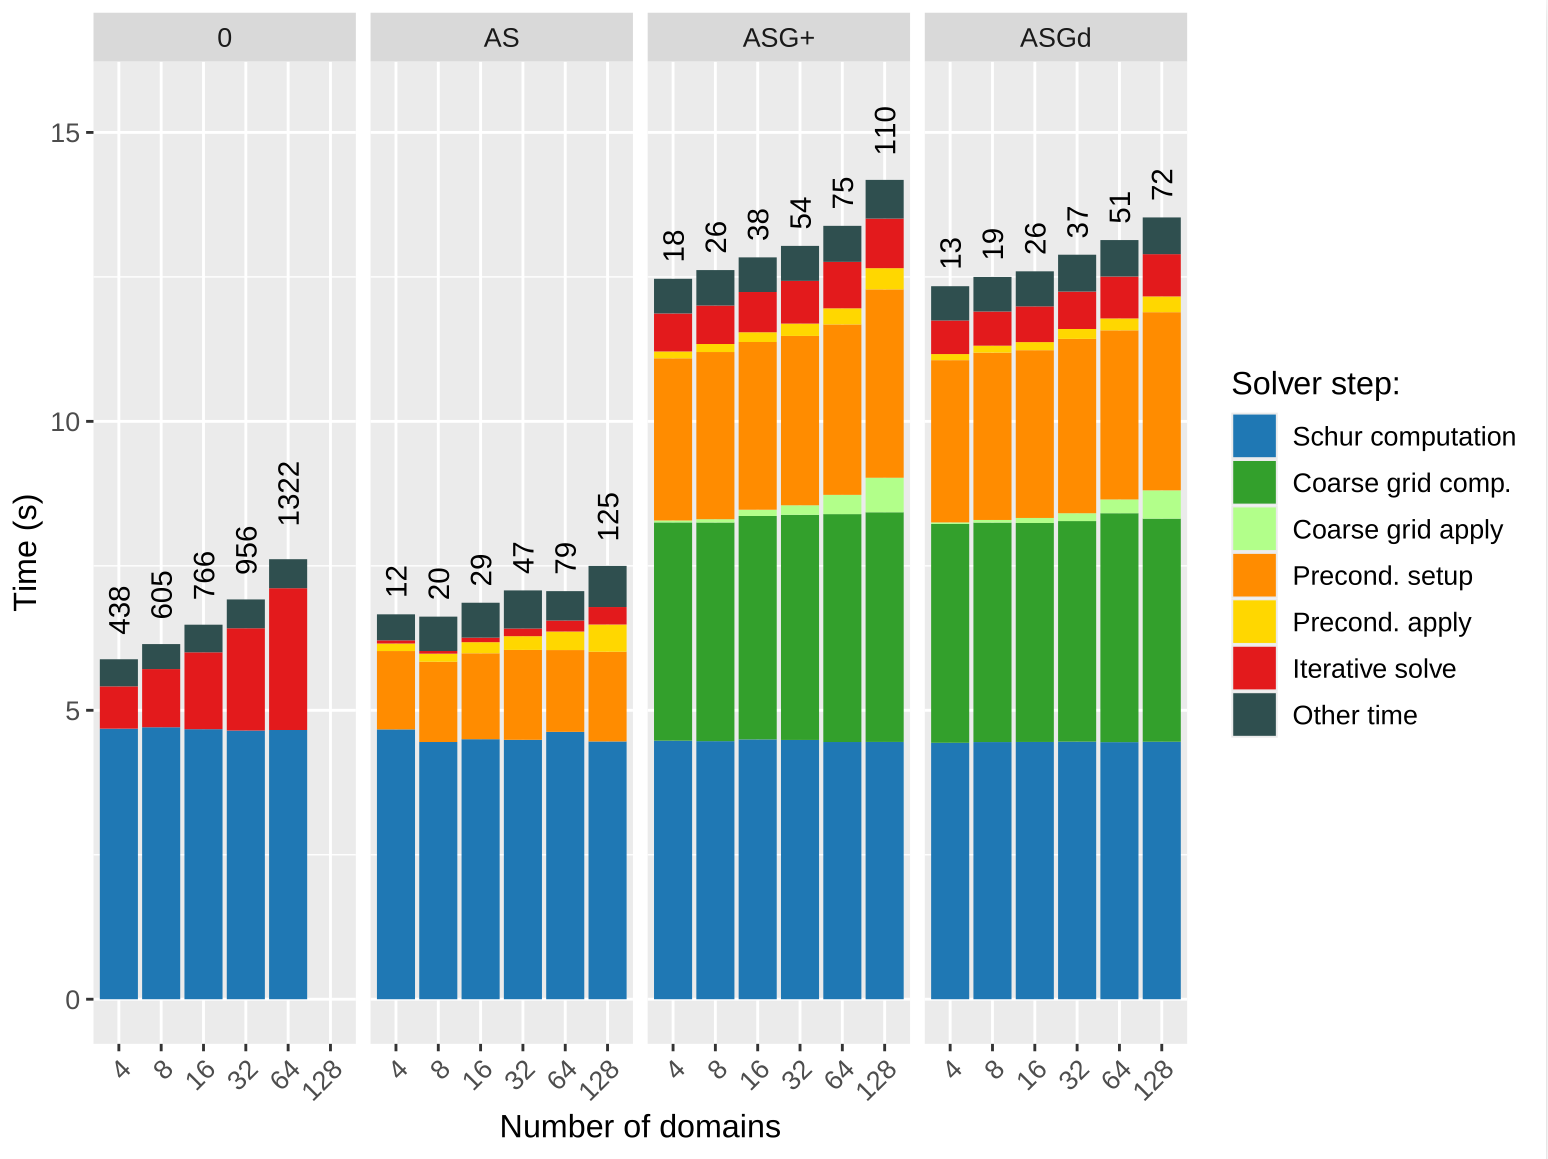
\includegraphics[width=0.8\textwidth]{graphics/composyx/results_jeanzay_S.png}
  \caption{Composyx weak scaling on Jean-Zay}
  \label{fig:composyx-jean-zay}
\end{figure}

On Figure \ref{fig:composyx-jean-zay}, we can see scaling results from
1 to 32 nodes, with 4 GPU v100 per node and one subdomain per GPU. We
can see for Additive Schwarz an efficiency of 88\%
($\frac{time(1 node)}{time(32 nodes)}$).  The
stopping criterion for this experiment is
$\frac{||b - A x ||}{||b||} = 10^{-8}$.

\paragraph{}
CUDA software stack is more complete than HIP's one. In particular,
the cuDSS library provides a sparse direct solver on GPU, which does
not have a counterpart for AMD where these type of computations have
to be made on CPU.
